% !TEX root = ../Thesis.tex

\chapter{Introduction}\
\label{ch:introduction}



\section{Motivation and Literature Review}\
\label{ch:motivation}
%(Context and justification, why is this work important?)\\

*paraphrase* Buildings are at the heart of society, and have a large impact on global health, economics and the environment. Europeans alone spend on average 90\% of their time in buildings \cite{Staniaszek2014BPIE} whether it be for work, rest or the multitude of activities that exists in modern society. *paraphrase* EU legislation new buildings. Significance for Switzerland.
Energy certification of existing buildings. Performative design of new buildings. Predicting the performance of refurbishments to assess return on investment. Two different types of simulation tools.
\item
Resistor Capacitor models as used in building physics. Earliest use, subsequent progress. Use in codes
Importance of the stochaistic term

% \\

%   \begin{figure}[ht] %h can be omitted for better page layout
%     \begin{center}
%       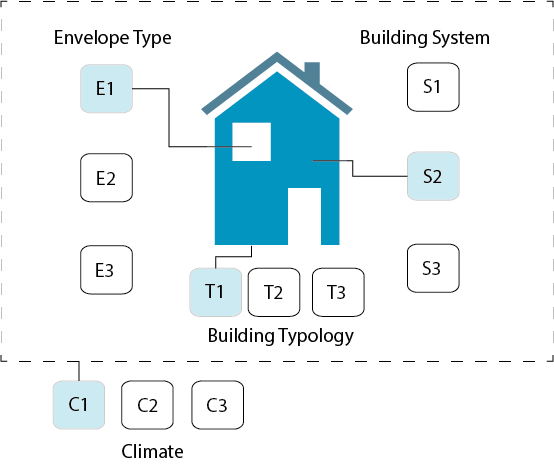
\includegraphics[width=\textwidth, trim= 0cm 0cm 0cm 0cm,clip]{envelope_system_comparison.png}
%       \caption{Figure Example}
%       \label{fig: comparison}
%     \end{center} 
%   \end{figure}

 
\section{Problem Statement}\
\begin{flushleft}
Because they inherently correct for imperfections and variations in the building fabric, stochaistic models are particularly useful when models need to be fitted to a building whose actual properties are unknown. 

Technologies such as the ASF need robust, accurate models to generate dynamic control inputs in real time.
	\item Simulation of existing buildings for retrofit purposes is time-consuming and not always accurate. An alternative would be a model that uses sensor data to self calibrate
	\item Traditional simulation approach is not good at describing short-time variations, which are important for control applications.
	\item Potential impacts: time savings in design, platform for innovative active integrated systems, more accurate models.
	\item Lack of transparency of source code when wanting to make modifications to test novel building technologies



\section{Objectives of Research}\
%(What do you want to achieve, more in general terms? Bullet point list)\\


	\item  A simple, robust, real-time model is needed to control increasingly complex building-integrated systems.
	\item 
		\item  model predictive control? - would require real-time weather forecasts

	\item  Find the best fitting model to sensor data to avoid running building simulations.

	\item  
		\item  OR: Use sensor data to calibrate adequately accurate model



\begin{itemize}
	\item Review literature and select appropriate models
	\item Set up an 1R-1C thermal model for a single zone as a learning exercise
	\item program 5R-2C thermal models as per ISO codes.
	\item Investigate options for discrete solvers
	
	\item Write good, transferable, open-source code in Python, making the program operable off linux (more reliable)
		\item Manage inputs
		\item output data in a useful and transferable format
	\item Validate the model:
		\item against physical data, possibly ASF and CP, or from existing datasets
		\item Against other models (physics based models) of the same building.
	\item Add complexity:	
		\item Create a graphical interface with a modular R-C model as input
		\item Set up PID controller for actuators (ASF) - requires model for ASF
		\item provide occupancy modelling ... (agent based?)
		\item use computer vision to compute effective window opening factor from photographs of facade and orientation OR just calculate from rhino geometry

\end{itemize}


\section{Thesis Outline}\
%Breakdown of your thesis (Not always necessary)


